%-----------------------------------------------------------------------------------------------------------------------------------------------%
%	The MIT License (MIT)
%
%	Copyright (c) 2020 Denish Azamuke
%
%	Permission is hereby granted, free of charge, to any person obtaining a copy
%	of this software and associated documentation files (the "Software"), to deal
%	in the Software without restriction, including without limitation the rights
%	to use, copy, modify, merge, publish, distribute, sublicense, and/or sell
%	copies of the Software, and to permit persons to whom the Software is
%	furnished to do so, subject to the following conditions:
%	
%	THE SOFTWARE IS PROVIDED "AS IS", WITHOUT WARRANTY OF ANY KIND, EXPRESS OR
%	IMPLIED, INCLUDING BUT NOT LIMITED TO THE WARRANTIES OF MERCHANTABILITY,
%	FITNESS FOR A PARTICULAR PURPOSE AND NONINFRINGEMENT. IN NO EVENT SHALL THE
%	AUTHORS OR COPYRIGHT HOLDERS BE LIABLE FOR ANY CLAIM, DAMAGES OR OTHER
%	LIABILITY, WHETHER IN AN ACTION OF CONTRACT, TORT OR OTHERWISE, ARISING FROM,
%	OUT OF OR IN CONNECTION WITH THE SOFTWARE OR THE USE OR OTHER DEALINGS IN
%	THE SOFTWARE.
%	
%
%-----------------------------------------------------------------------------------------------------------------------------------------------%


%============================================================================%
%
%	DOCUMENT DEFINITION
%
%============================================================================%

%we use article class because we want to fully customize the page and don't use a cv template
\documentclass[10pt,A4]{article}	


%----------------------------------------------------------------------------------------
%	ENCODING
%----------------------------------------------------------------------------------------

% we use utf8 since we want to build from any machine
\usepackage[utf8]{inputenc}		

%----------------------------------------------------------------------------------------
%	LOGIC
%----------------------------------------------------------------------------------------

% provides \isempty test
\usepackage{xstring, xifthen}

%----------------------------------------------------------------------------------------
%	FONT BASICS
%----------------------------------------------------------------------------------------

% some tex-live fonts - choose your own

%\usepackage[defaultsans]{droidsans}
%\usepackage[default]{comfortaa}
%\usepackage{cmbright}
\usepackage[default]{raleway}
%\usepackage{fetamont}
%\usepackage[default]{gillius}
%\usepackage[light,math]{iwona}
%\usepackage[thin]{roboto} 

% set font default
\renewcommand*\familydefault{\sfdefault} 	
\usepackage[T1]{fontenc}

% more font size definitions
\usepackage{moresize}

%----------------------------------------------------------------------------------------
%	FONT AWESOME ICONS
%---------------------------------------------------------------------------------------- 

% include the fontawesome icon set
\usepackage{fontawesome}

% use to vertically center content
% credits to: http://tex.stackexchange.com/questions/7219/how-to-vertically-center-two-images-next-to-each-other
\newcommand{\vcenteredinclude}[1]{\begingroup
\setbox0=\hbox{\includegraphics{#1}}%
\parbox{\wd0}{\box0}\endgroup}

% use to vertically center content
% credits to: http://tex.stackexchange.com/questions/7219/how-to-vertically-center-two-images-next-to-each-other
\newcommand*{\vcenteredhbox}[1]{\begingroup
\setbox0=\hbox{#1}\parbox{\wd0}{\box0}\endgroup}

% icon shortcut
\newcommand{\icon}[3] { 							
	\makebox(#2, #2){\textcolor{maincol}{\csname fa#1\endcsname}}
}	

% icon with text shortcut
\newcommand{\icontext}[4]{ 						
	\vcenteredhbox{\icon{#1}{#2}{#3}}  \hspace{2pt}  \parbox{0.9\mpwidth}{\textcolor{#4}{#3}}
}

% icon with website url
\newcommand{\iconhref}[5]{ 						
    \vcenteredhbox{\icon{#1}{#2}{#5}}  \hspace{2pt} \href{#4}{\textcolor{#5}{#3}}
}

% icon with email link
\newcommand{\iconemail}[5]{ 						
    \vcenteredhbox{\icon{#1}{#2}{#5}}  \hspace{2pt} \href{mailto:#4}{\textcolor{#5}{#3}}
}

%----------------------------------------------------------------------------------------
%	PAGE LAYOUT  DEFINITIONS
%----------------------------------------------------------------------------------------

% page outer frames (debug-only)
% \usepackage{showframe}		

% we use paracol to display breakable two columns
\usepackage{paracol}

% define page styles using geometry
\usepackage[a4paper]{geometry}

% remove all possible margins
\geometry{top=1cm, bottom=1cm, left=1cm, right=1cm}

\usepackage{fancyhdr}
\pagestyle{empty}

% space between header and content
% \setlength{\headheight}{0pt}

% indentation is zero
\setlength{\parindent}{0mm}

%----------------------------------------------------------------------------------------
%	TABLE /ARRAY DEFINITIONS
%---------------------------------------------------------------------------------------- 

% extended aligning of tabular cells
\usepackage{array}

% custom column right-align with fixed width
% use like p{size} but via x{size}
\newcolumntype{x}[1]{%
>{\raggedleft\hspace{0pt}}p{#1}}%


%----------------------------------------------------------------------------------------
%	GRAPHICS DEFINITIONS
%---------------------------------------------------------------------------------------- 

%for header image
\usepackage{graphicx}

% use this for floating figures
% \usepackage{wrapfig}
% \usepackage{float}
% \floatstyle{boxed} 
% \restylefloat{figure}

%for drawing graphics		
\usepackage{tikz}				
\usetikzlibrary{shapes, backgrounds,mindmap, trees}

%----------------------------------------------------------------------------------------
%	Color DEFINITIONS
%---------------------------------------------------------------------------------------- 
\usepackage{transparent}
\usepackage{color}

% primary color
\definecolor{maincol}{RGB}{ 225, 0, 0 }

% accent color, secondary
% \definecolor{accentcol}{RGB}{ 250, 150, 10 }

% dark color
\definecolor{darkcol}{RGB}{ 70, 70, 70 }

% light color
\definecolor{lightcol}{RGB}{245,245,245}


% Package for links, must be the last package used
\usepackage[hidelinks]{hyperref}

% returns minipage width minus two times \fboxsep
% to keep padding included in width calculations
% can also be used for other boxes / environments
\newcommand{\mpwidth}{\linewidth-\fboxsep-\fboxsep}
	


%============================================================================%
%
%	CV COMMANDS
%
%============================================================================%

%----------------------------------------------------------------------------------------
%	 CV LIST
%----------------------------------------------------------------------------------------

% renders a standard latex list but abstracts away the environment definition (begin/end)
\newcommand{\cvlist}[1] {
	\begin{itemize}{#1}\end{itemize}
}

%----------------------------------------------------------------------------------------
%	 CV TEXT
%----------------------------------------------------------------------------------------

% base class to wrap any text based stuff here. Renders like a paragraph.
% Allows complex commands to be passed, too.
% param 1: *any
\newcommand{\cvtext}[1] {
	\begin{tabular*}{1\mpwidth}{p{0.98\mpwidth}}
		\parbox{1\mpwidth}{#1}
	\end{tabular*}
}

%----------------------------------------------------------------------------------------
%	CV SECTION
%----------------------------------------------------------------------------------------

% Renders a a CV section headline with a nice underline in main color.
% param 1: section title
\newcommand{\cvsection}[1] {
	\vspace{14pt}
	\cvtext{
		\textbf{\LARGE{\textcolor{darkcol}{\uppercase{#1}}}}\\[-4pt]
		\textcolor{maincol}{ \rule{0.1\textwidth}{2pt} } \\
	}
}

%----------------------------------------------------------------------------------------
%	META SKILL
%----------------------------------------------------------------------------------------

% Renders a progress-bar to indicate a certain skill in percent.
% param 1: name of the skill / tech / etc.
% param 2: level (for example in years)
% param 3: percent, values range from 0 to 1
\newcommand{\cvskill}[3] {
	\begin{tabular*}{1\mpwidth}{p{0.72\mpwidth}  r}
 		\textcolor{black}{\textbf{#1}} & \textcolor{maincol}{#2}\\
	\end{tabular*}%
	
	\hspace{4pt}
	\begin{tikzpicture}[scale=1,rounded corners=2pt,very thin]
		\fill [lightcol] (0,0) rectangle (1\mpwidth, 0.15);
		\fill [maincol] (0,0) rectangle (#3\mpwidth, 0.15);
  	\end{tikzpicture}%
}


%----------------------------------------------------------------------------------------
%	 CV EVENT
%----------------------------------------------------------------------------------------

% Renders a table and a paragraph (cvtext) wrapped in a parbox (to ensure minimum content
% is glued together when a pagebreak appears).
% Additional Information can be passed in text or list form (or other environments).
% the work you did
% param 1: time-frame i.e. Sep 14 - Jan 15 etc.
% param 2:	 event name (job position etc.)
% param 3: Customer, Employer, Industry
% param 4: Short description
% param 5: work done (optional)
% param 6: technologies include (optional)
% param 7: achievements (optional)
\newcommand{\cvevent}[7] {
	
	% we wrap this part in a parbox, so title and description are not separated on a pagebreak
	% if you need more control on page breaks, remove the parbox
	\parbox{\mpwidth}{
		\begin{tabular*}{1\mpwidth}{p{0.72\mpwidth}  r}
	 		\textcolor{black}{\textbf{#2}} & \colorbox{maincol}{\makebox[0.25\mpwidth]{\textcolor{white}{#1}}} \\
			\textcolor{maincol}{\textbf{#3}} & \\
		\end{tabular*}\\[8pt]
	
		\ifthenelse{\isempty{#4}}{}{
			\cvtext{#4}\\
		}
	}

	\ifthenelse{\isempty{#5}}{}{
		\vspace{9pt}
		{#5}
	}

	\ifthenelse{\isempty{#6}}{}{
		\vspace{9pt}
		\cvtext{\textbf{Technologies include:}}\\
		{#6}
	}

	\ifthenelse{\isempty{#7}}{}{
		\vspace{9pt}
		\cvtext{\textbf{Achievements include:}}\\
		{#7}
	}
	\vspace{14pt}
}

%----------------------------------------------------------------------------------------
%	 CV META EVENT
%----------------------------------------------------------------------------------------

% Renders a CV event on the sidebar
% param 1: title
% param 2: subtitle (optional)
% param 3: customer, employer, etc,. (optional)
% param 4: info text (optional)
\newcommand{\cvmetaevent}[4] {
	\textcolor{maincol} {\cvtext{\textbf{\begin{flushleft}#1\end{flushleft}}}}

	\ifthenelse{\isempty{#2}}{}{
	\textcolor{darkcol} {\cvtext{\textbf{#2}} }
	}

	\ifthenelse{\isempty{#3}}{}{
		\cvtext{{ \textcolor{darkcol} {#3} }}\\
	}

	\cvtext{#4}\\[14pt]
}




%============================================================================%
%
%
%
%	DOCUMENT CONTENT
%
%
%
%============================================================================%
\begin{document}
\columnratio{0.31}
\setlength{\columnsep}{2.2em}
\setlength{\columnseprule}{4pt}
\colseprulecolor{lightcol}
\begin{paracol}{2}
\begin{leftcolumn}
%---------------------------------------------------------------------------------------
%	META IMAGE
%----------------------------------------------------------------------------------------
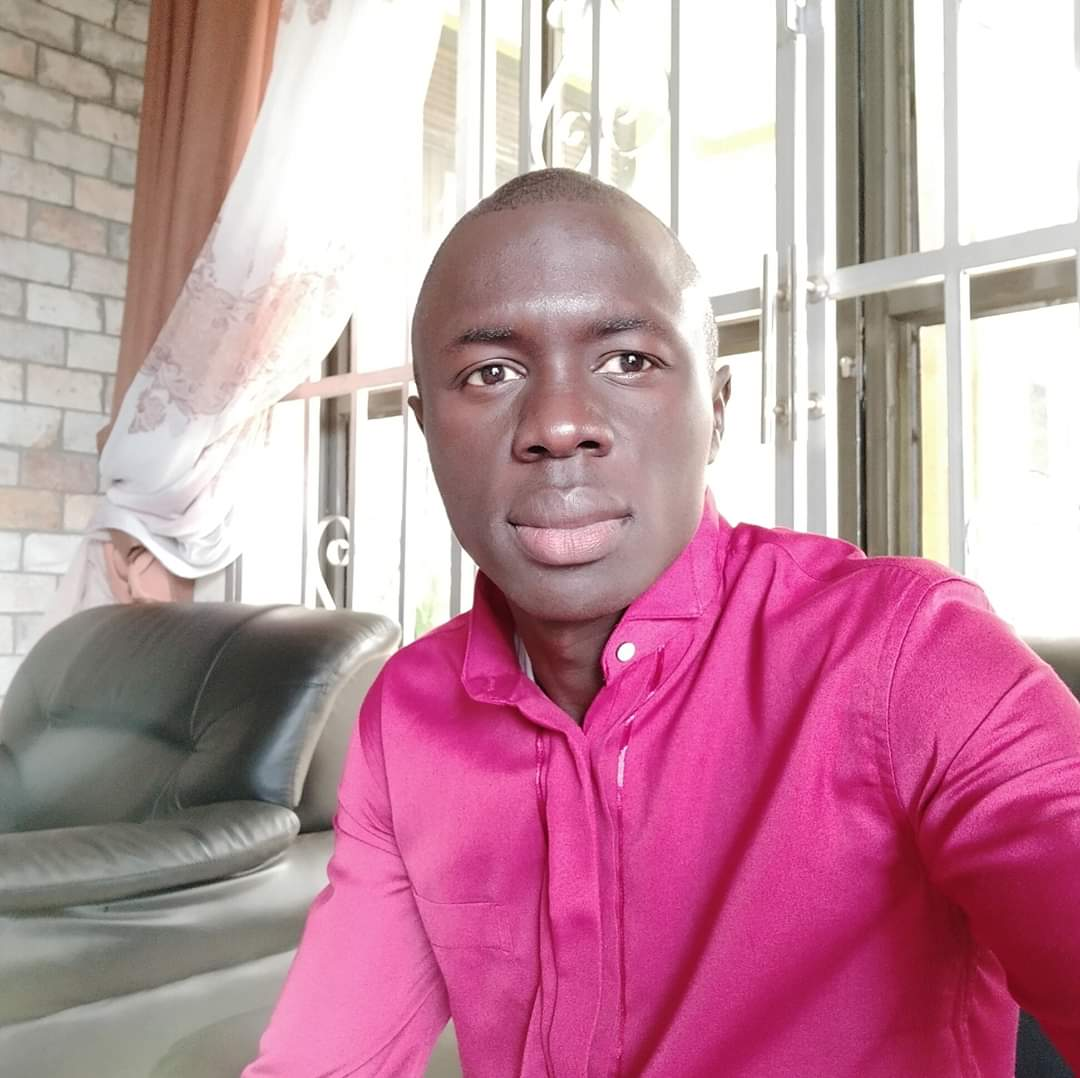
\includegraphics[width=\linewidth]{untitled.jpg}	%trimming relative to image size

%---------------------------------------------------------------------------------------
%	PERSONAL DATA
%----------------------------------------------------------------------------------------
\cvsection{PERSONAL DATA}

\cvmetaevent
{Date of Birth}
{}
{}
{$16^{th}$ Feb 1998}

\cvmetaevent
{Nationality}
{}
{}
{Ugandan}
\cvmetaevent
{Gender}
{}
{}
{Male}


%---------------------------------------------------------------------------------------
%	META SKILLS
%----------------------------------------------------------------------------------------
\cvsection{SKILLS}

\cvskill{Project Management} {3+ yrs} {1} \\[-2pt]

\cvskill{Enterprise Softwares} {3+ yrs} {0.97} \\[-2pt]

\cvskill{Latex} {2+ yrs} {1} \\[-2pt]

\cvskill{Cloud Computing} {3+ yrs} {0.9} \\[-2pt]


\cvskill{Research} {3+ yrs} {0.9} \\[-2pt]

\cvskill{System Administration} {2+ yrs} {0.85} \\[-2pt]



\cvskill{Programming (Python, Java)} {2+ yrs} {0.8} \\[-2pt]

\cvskill{Team building} {2+ yrs} {0.69} \\[-2pt]

\cvskill{Change management} {1+ yrs} {0.6} \\[-2pt]






\vfill
%\cvqrcode{0.7}


%---------------------------------------------------------------------------------------
%	EDUCATION
%----------------------------------------------------------------------------------------
%\newpage
\cvsection{EDUCATION}

\cvmetaevent
{2016 - 2019}
{BSc. Computer Science.}
{Makerere University}
{Main thematic priority of the bachelor studies was using computational techniques to solve most of the prevailing community problems and hence supporting the industry.\\\\In the undergraduate project, my research limited itself to a mechanism in which Boda boda riders and Motorists borrow fuel and further save their money within the application specifically for fuel. The idea was to give credit fuel service to the users and allow them pay within three days with a small service fee. This innovation (mobile application) addressed the major challenge of not having fuel to start your journey.\\\\Graduated with \textbf{Second Class Honors (Upper Division), CGPA of 4.16} out of 5.0}

\cvmetaevent
{2014 - 2015}
{Uganda Advanced Certificate of Education (UACE).}
{St. Mary's ss Kitende}
{The subjects for this level were:
	 \textbf{Physics, Chemistry, Mathemeatics and Subsidiary ICT.} Excelled with \textbf{17 points} out of 20 points.} \\\\Also Studied lower elementary education:\textbf{ UCE and PLE}, obtained \textbf{top grades} 

\vfill\null
%\cvqrcode{0.7}

%---------------------------------------------------------------------------------------
%	WORKSHOPS
%----------------------------------------------------------------------------------------
%\newpage
\cvsection{WORKSHOPS}

\cvmetaevent
{Azure Infrastructure as a Service}
{}
{}
{Certificate issued by Microsoft to prove abilities in Exchange online Administration and Configuration}

\cvmetaevent
{Azure Software as a Service}
{}
{}
{Certificate issued by Microsoft to prove abilities in using enterprise cloud softwares as a service, case study was Azure SaaS for the National Social Security Fund (NSSF) Uganda}


\cvmetaevent
{Africa Block Chain Conference}
{}
{}
{A talk on Blockchain technology, preparing Africa for the $4^{th}$ industrial revolution.\\I was part of the team that represented Makerere University in that event held on July $3^{rd}$ - $4^{th}$, 2019 at Kampala Serena Hotel }


\cvmetaevent
{Online Classes}
{}
{}
{It is important for me to stay up to date with the newest topics in the field of IT. In DevOps it is also important to have a general overview and a hands-on experience on them. Therefore, besides intense article studies, I also keep myself up to date with online classes.}

\vfill
%\cvqrcode{0.7}



%---------------------------------------------------------------------------------------
%	LANGUAGES
%----------------------------------------------------------------------------------------
%\newpage
\cvsection{LANGUAGES}

\cvmetaevent
{Engilish}
{}
{}
{Fluent}

\cvmetaevent
{Lugbara}
{}
{}
{Fluent}


\cvmetaevent
{Kiswahili}
{}
{}
{Intermidiate}


\cvmetaevent
{Luganda}
{}
{}
{Intermidiate}

\newpage

\vfill
%\cvqrcode{0.7}
%---------------------------------------------------------------------------------------
%	CONTACT
%----------------------------------------------------------------------------------------
\vfill\null
\cvsection{CONTACT}

\icontext{MapMarker}{12}{Kasangati Town Council\\Nangabo Village}{black}\\[6pt]
\icontext{MobilePhone}{12}{+256 789 061 019}{black}\\[6pt]
\iconemail{Envelope}{12}{denishazamuke@gmail.com}{denishazamuke@gmail.com}{black}\\[6pt]
{https://azamukedenish.github.io}\\[6pt]

\vfill\null
%\cvqrcode{0.7}




\newpage
\mbox{} % hotfix to place qrcode on the bottom when there are not other elements
\vfill
%\cvqrcode{0.7}

\end{leftcolumn}
\begin{rightcolumn}
%---------------------------------------------------------------------------------------
%	TITLE  HEADER
%----------------------------------------------------------------------------------------
\fcolorbox{white}{darkcol}{\begin{minipage}[c][3.5cm][c]{1\mpwidth}
	\begin {center}
		\HUGE{ \textbf{ \textcolor{white}{ \uppercase{ AZAMUKE DENISH } } } } \\[-24pt]
		\textcolor{white}{ \rule{0.1\textwidth}{1.25pt} } \\[4pt]
		\large{ \textcolor{white} {Practical IT officer and Developer Advocate} }
	\end {center}
\end{minipage}} \\[14pt]
\vspace{-12pt}

%---------------------------------------------------------------------------------------
%	PROFILE
%----------------------------------------------------------------------------------------
\vfill\null
\cvsection{PROFILE}

\cvtext{IT Officer with strong enterprise skills, driven by passion for troubleshooting and giving solutions for IT problems at Enterprise level.\\

Developer Advocacy, specialized both in automation and adopting latest technologies for the enterprise, experienced in managing enterprise systems and heterogeneous infrastructures. The link between development and operations, comfortable in both.\\

Customer-oriented and structured method of working, focused on quality and maintainability. Highly motivated to work in a team, both comfortable in big companies as in small teams.\\

}

%---------------------------------------------------------------------------------------
%	WORK EXPERIENCE
%----------------------------------------------------------------------------------------
\vfill\null
\cvsection{WORK EXPERIENCE}

\cvevent
	{Jan 2020 - NOW}
	{Data Scientist}
	{National Social Security Fund (NSSF) Uganda}
	{A large data analysis and visualization project for making decisions for procuring items for NSSF Uganda. This project limited itself to extraction of data from the source systems at the department of Procurement and Disposal Unit, data cleaning and transformation to make cost effective decisions for the Fund.}
	{\cvlist{
		\item Data collection and extraction
		\item Data cleaning
		\item Data transformation
		\item  Enterprise decision making 
	}}
	{\cvlist {
		\item Google forms and survey monkey- for data collection
		\item Anaconda distribution software package for data extraction, cleaning and visualisation
		\item Python programming language and Matplotlib library for ploting graphs
		\item Latex for professional documentation
	}}
	{\cvlist{
		\item Online record of data
		\item Informed decision making
		\item Enterprise research experience
	}}


\vfill\null
\cvevent
{Sep 18 - Dec 19}
{IT Consultant}
{Ignition Ventures Limited}
{Large public service project with the goal to establish a platform for handling of finance processes with a very high number of transactions. Main focus was the migration of legacy data, by assuring data quality and transformation into various formats}
{\cvlist{
		\item Customer consulting with regard to loading / unloading interfaces
		\item Definition of requirements for transformation of legacy data
		\item Implementation of algorithms for data transformation
		\item Tool development for secure data transport
		\item Tool development for tests of data quality/interface implementation
}}
{\cvlist {
		\item Standard Linux tools, such as awk, sed, grep
		\item Python for in-depth data analysis
		\item Java for transport layers
		\item IBM DataStage
}}
{\cvlist{
		\item Definition of uniform standards
		\item Introduction of the standard Linux stack as global toolset for data analysis in project
}}

\vfill\null
\cvevent
	{Jun 18 - Aug 18}
	{Junior IT Officer}
	{National Social Security Fund (NSSF) Uganda}
	{Responsible for infrastructure architecture / automaton as well as custom software development on a project for contracts management in a large heterogeneous environment.}
	{\cvlist{
		\item Design and implementation of web based contracts management system
		\item Incident management and documentation
		\item Customized tool creation for the contracts management system
		\item Enterprise software Installation using Windows Deployment Service (WDS)
		\item Troubleshooting computer systems
		\item IT system administration
		\item Customer support in IT related problems
		\item User training and overall education
		\item Management of enterprise cloud infrastructure
		\item Adding/removing users on network and Active directory management
		\item Introduction to enterprise database configuration and management
		\item Enterprise research and e-learning
	}}
	{\cvlist {
		\item Service Now for incident management 
		\item Python for custom tool development
		\item WDS for enterprise software installation
		\item Git for configuration and documentation versioning
		\item Google forms for enterprise research
		\item Oracle databases for database configuration and management
		\item Fortnet for computer networking
	}}
	{\cvlist{
		\item Drastically accelerated (~20x faster) the contracts follow up process and improved its reliability by introducing dynamic web based contracts management system
		\item Deployed several softwares in short time to many computers
		\item Experience in reliable incident management
		\item Change management skills through user education
		\item IT research skills		
	}}





\newpage

%---------------------------------------------------------------------------------------
%	REFEREES
%----------------------------------------------------------------------------------------
\vfill\null
\cvsection{REFEREES}

\cvtext{\textbf{Prof. Engineer Bainomugisha}\\
	
	Head, Department of Computer Science,\\
	School of Computing and Information Sciences,\\
	Makerere University\\
		\icontext{MobilePhone}{12}{+256 Add your own}{black}\\[6pt]
	\iconemail{Envelope}{12}{Add your own}{Add your own}{black}\\[6pt]

	
}\\\\

\cvtext{\textbf{Bitwire Gorge Albert}\\
	
	Assistant Lecturer, Department of Information Technology,\\
	School of Computing and Information Sciences,\\
	Makerere University\\	
	\icontext{MobilePhone}{12}{+256 Add your own}{black}\\[6pt]
	\iconemail{Envelope}{12}{Add your own}{Add your own}{black}\\[6pt]
}\\\\

\cvtext{\textbf{Kyeyune Godfrey}\\
	
	Applications Developer, Department of Infromation Technology,\\National Social Security Fund (NSSF) Uganda\\
	\icontext{MobilePhone}{12}{+256 Add your own}{black}\\[6pt]
	\iconemail{Envelope}{12}{Add your own}{Add your own}{black}\\[6pt]
}

\textbf{NOTE: This template was developed using \LaTeX, please customise with your own data.}
\newpage
\end{rightcolumn}
\end{paracol}
\end{document}

